% !TEX root = ./Research_and_SA.tex

\textbf{SIGNIFICANCE}
RNA lies at the center of cellular function. Its most appreciated function is to carry protein blueprints from the genetic code of the nucleus to be manufactured into the protein machines of the cell at the ribosome. Only recently have researchers begun to appreciate its myriad of other functions, many of which also lie at the center of important cellular processes. \comment{X, Y, and Z (maybe the proposed test systems??)} have been recently found to have crucial RNA components. This importance for cellular function necessitates a toolset of probes to study these RNAs as they traverse the cell. Indeed, the location of these RNA transcripts has been implicated to be instrumental in their function.\cite{Muller-McNicollHowcellsget2013a}

Proteins benefit from a large imaging toolkit that has been developed over the last \comment{XX} years. Genetically encodable fluorescent proteins are now ubiquitous for the study of the localization of any translated target in the cell. 

%%%%%%%%%%%%%%%%%%%%%%%%%%%%%%%%%%%%%%%%%%%%%%%%%%%%%%%%%%%%%%%%%%%%%%%%%%%%%%%%
%Riboglow
\begin{wrapfigure}[18]{r}{10cm}
%\vspace{-0.2in}
\begin{centering}
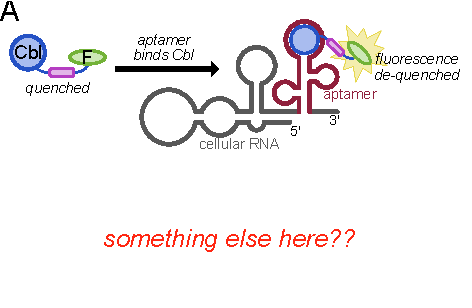
\includegraphics[width=\textwidth]{figures/fig1.pdf}

\end{centering}
\footnotesize
\caption{\label{figure:riboglow}
A) Cobalamin acts as a quenching and localization moiety to guide a fluorescent probe to an RNA transcript of interest. When unbound, fluorescence is quenched. In the presence of RNA tagged with the cobalamin aptamer, fluorescence is restored.
}
\end{wrapfigure}
%%%%%%%%%%%%%%%%%%%%%%%%%%%%%%%%%%%%%%%%%%%%%%%%%%%%%%%%%%%%%%%%%%%%%%%%%%%%%%%%

\textbf{BACKGROUND}
Lorem ipsum dolor sit amet, consectetur adipisicing elit, sed do eiusmod tempor incididunt ut labore et dolore magna aliqua. Ut enim ad minim veniam, quis nostrud exercitation ullamco laboris nisi ut aliquip ex ea commodo consequat. Duis aute irure dolor in reprehenderit in voluptate velit esse cillum dolore eu fugiat nulla pariatur. Excepteur sint occaecat cupidatat non proident, sunt in culpa qui officia deserunt mollit anim id est laborum.

Lorem ipsum dolor sit amet, consectetur adipisicing elit, sed do eiusmod tempor incididunt ut labore et dolore magna aliqua. Ut enim ad minim veniam, quis nostrud exercitation ullamco laboris nisi ut aliquip ex ea commodo consequat. Duis aute irure dolor in reprehenderit in voluptate velit esse cillum dolore eu fugiat nulla pariatur. Excepteur sint occaecat cupidatat non proident, sunt in culpa qui officia deserunt mollit anim id est laborum.

\textbf{APPROACH \underline{Aim 1.} Synthesize improved Riboglow probes.}\\
The main drawback of Riboglow is the poor turn-on that is observed upon probe binding. In this aim, I intend to leverage my background in synthetic chemistry to produce a panel of diverse probe structures that improve fluorescence quenching (and thus signal induction). In previous studies in collaboration with Professor Dorota Gryko (see Gryko letter of support) a small number of linkers and fluorophores were evaluated for quenching and fluorescence turn-on. Linker length and fluorophore wavelength were varied to gauge the quenching ability of cobalamin. Though some degree of quenching occurred in all of the constructs synthesized, the best probes always had the shortest linkers. Intuitively, the shortest linkers also gave the poorest fluorescence induction.
%Unfortunately, the best probes were also the fluorophores with the shortest emission wavelengths.
\textit{To increase quenching I will vary linker composition to maximize quenching in the unbound state, and minimize it in the bound state.} Ideally, in the unbound state, the cobalamin and the fluorophore would be closely associated to maximize FRET and contact quenching.\cite{LeeDesignSynthesisCharacterization2009} In the bound state, the molecules would reside at their maximal distance to promote fluorescence. To strike this balance, I propose the use of a synthetic beta turn as the linker between cobalamin and the fluorophore. Such a linker would hold the molecules close in solution, but would be linearized upon binding to the aptamer. A number of such beta turns have been developed. These motifs are as small as twelve amino acids and many are stable to denaturation up to 85 C.\cite{KierProbingLowerSize2008} In the unbound state, such a linker would hold the quencher and fluorophore in close proximity (due to the short distance between the N and C termini of the peptide). When the cobalamin is bound by an aptamer, steric occlusion would force the beta turn to unfold to place the fluorophore-quencher pair at a larger distance. The amino acids of the peptide linker will be varied to adjust the stability of the fold.

\textbf{\underline{Aim 2.} Adapt Riboglow for superresolution imaging.}\\
Lorem ipsum dolor sit amet, consectetur adipisicing elit, sed do eiusmod tempor incididunt ut labore et dolore magna aliqua. Ut enim ad minim veniam, quis nostrud exercitation ullamco laboris nisi ut aliquip ex ea commodo consequat. Duis aute irure dolor in reprehenderit in voluptate velit esse cillum dolore eu fugiat nulla pariatur. Excepteur sint occaecat cupidatat non proident, sunt in culpa qui officia deserunt mollit anim id est laborum.

%%%%%%%%%%%%%%%%%%%%%%%%%%%%%%%%%%%%%%%%%%%%%%%%%%%%%%%%%%%%%%%%%%%%%%%%%%%%%%%%
%Multicomponent
\begin{wrapfigure}[25]{l}{10cm}
%\vspace{-0.2in}
\begin{centering}
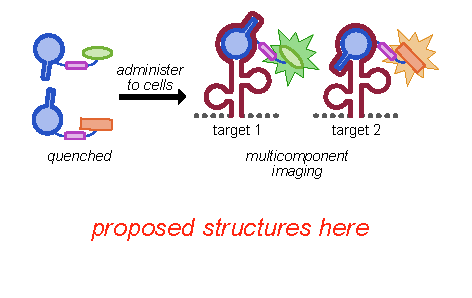
\includegraphics[width=\textwidth]{figures/fig3.pdf}

\end{centering}
\footnotesize
\caption{\label{figure:multicomponent}
A) Mutually orthogonal cobalamin analogs will enable multicomponent RNA imaging. Signal turn-on will only be observed in the presence of the matched pair. B)\comment{Propose some structures.} C) SELEX will be used to screen for aptamers that bind each cobalamin in a mutually-exclusive manner.
}
\end{wrapfigure}
%%%%%%%%%%%%%%%%%%%%%%%%%%%%%%%%%%%%%%%%%%%%%%%%%%%%%%%%%%%%%%%%%%%%%%%%%%%%%%%%

\textbf{\underline{Aim 3.} Develop mutually orthogonal Riboglow probes for multicomponent imaging.}\\
Lorem ipsum dolor sit amet, consectetur adipisicing elit, sed do eiusmod tempor incididunt ut labore et dolore magna aliqua. Ut enim ad minim veniam, quis nostrud exercitation ullamco laboris nisi ut aliquip ex ea commodo consequat. Duis aute irure dolor in reprehenderit in voluptate velit esse cillum dolore eu fugiat nulla pariatur. Excepteur sint occaecat cupidatat non proident, sunt in culpa qui officia deserunt mollit anim id est laborum.

%%% Local Variables: ***
%%% mode: latex ***
%%% TeX-master: "Research_and_SA.tex" ***
%%% End: ***
